%
% 建议用 pdflatex 编译
%
\documentclass{article}

%%%%%===== 页面设置 =====================================================
\usepackage[a4paper,top=2.54cm,bottom=2.54cm,left=3.17cm,right=3.17cm,%
            includehead,includefoot]{geometry}

%%%%%===== 常用宏包 =====================================================
\usepackage{amsmath,amssymb,amsfonts,amsthm}
\usepackage{siunitx}
\usepackage{tikz}
\usepackage{pgfplots}
\pgfplotsset{compat=1.18}
\usepackage{pifont}
\usepackage{graphicx}
\usepackage{subcaption}
\usepackage{float}
\usepackage{xcolor}
\usepackage[numbers,square,sort&compress]{natbib}
\usepackage{hyperref}
  \hypersetup{colorlinks,citecolor=blue,linkcolor=blue,breaklinks=true}
\usepackage{booktabs}
\usepackage{colortbl}
\usepackage{caption}
\usepackage{enumitem}
\usepackage{epstopdf}
\usepackage{algorithm}
\usepackage{algpseudocode}
\usepackage{array}
\usepackage{bbding}
\usepackage{fancyhdr} % 页眉
\usepackage{fancyvrb} % 摘录 Verbatim 环境
\usepackage{longtable}
\usepackage{listings}
\usepackage{rotating,rotfloat} % 提供 sidewayfigure 和 sidewaystable 环境横排图表
\usepackage{yhmath} % \wideparen 弧 \adots

%%%%%===== 页眉页脚 =====================================================
\usepackage{fancyhdr}
\pagestyle{fancy}
\fancyhf{}
\renewcommand{\headrulewidth}{0pt}
\renewcommand{\sectionmark}[1]{\markboth{\uppercase{#1}}{}}
\chead{\leftmark}
\cfoot{\thepage}

%%%%%===== 行间距 ======================================================
\renewcommand{\baselinestretch}{1.1}

%%%%%===== 数学公式 =====================================================
\allowdisplaybreaks

%%%%%===== 定义定理 =====================================================
\newtheorem{theorem}{Theorem}[section]
\newtheorem{lemma}{Lemma}[section]
\newtheorem{corollary}[theorem]{Corollary}
\newtheorem{proposition}[theorem]{Proposition}
\newtheorem{definition}{Definition}[section]
\newtheorem{example}{Example}
\newtheorem{remark}{Remark}

%%%%%===== 自定义命令 ====================================================
\newcommand{\R}{\mathbb{R}}
\newcommand{\dis}{\displaystyle}


\DeclareMathOperator{\diag}{diag}

\begin{document}

\title{A Note on 1D Riemann Problem for the Reactive Flow}

\author{
  Yu Xingchun
}

\date{\today}

\maketitle

\begin{abstract}

\end{abstract}


\section{Riemann Problem}
\subsection{The governing equations}
The reactive Euler equations in one-dimensional space can be expressed as the classical Euler equations supplemented by a chemical reaction term, i.e.,
\begin{equation}
\partial_t \mathbf{U} + \partial_x \mathbf{F}(\mathbf{U}) = \mathbf{S}(\mathbf{U}),
\end{equation}
with
\begin{equation}
\boldsymbol{U} = \begin{bmatrix} \rho \\ \rho u \\ E \\ \rho \lambda \end{bmatrix}, \quad
\boldsymbol{F} = \begin{bmatrix} \rho u \\ \rho u^2 + p \\  (E+p)u \\ \rho u \lambda  \end{bmatrix}, \quad
\boldsymbol{S} = \begin{bmatrix} 0 \\ 0 \\ 0 \\ \rho \lambda K\end{bmatrix}.
\end{equation}
In this system,
\begin{itemize}
  \item $\rho$ is the density,
  \item $u$ is the velocity,
  \item $E$ is the total energy,
  \item $p$ is the pressure,
  \item $\lambda$ is the mass fraction of the unburnt gas,
  \item $K$ is the chemical reaction rate.
\end{itemize}
The total energy $E$ is given by
\begin{equation}
E = \rho \varepsilon + \frac{1}{2} \rho u^2,
\end{equation} 
where $\varepsilon$ is the internal energy.

The equation of state is given with the ideal gas,
\begin{equation}
\epsilon  = \frac{p}{(\gamma - 1) \rho} + (1-\lambda) q_b + \lambda q_u,
\label{eq:EOS}
\end{equation}
where $q_b$ (resp. $q_u$) are chemical energy of the burnt (resp. unburnt) gas, and $\gamma$ is the polytropic index.
According to the equation of state, the speed of sound 
$c$ is given by the following expression:
\begin{equation}
  c^2 = \frac{\partial p}{\partial \rho}+\frac{p}{\rho^2}\frac{\partial p}{\partial e}
  = \frac{\gamma(p)}{\rho}.
\end{equation}

For an exothermic reaction, $q_b < q_u$. We denote 
\[
\Delta = q_b - q_u <0.
\]

\subsection{Champman-Jouguet (CJ) Model}
The Chapman-Jouguet (CJ) model is a simplified framework for modeling reactive flows. It is based on the following key assumptions:
\begin{enumerate}
  \item The flow is one-dimensional, and the effects of viscosity, species diffusion, and heat conduction are neglected.
  \item The chemical reaction is assumed to occur infinitely fast, such that thermochemical equilibrium is achieved instantaneously.
  \item The reactive front is treated as a discontinuity, which is conservative and satisfies the Rankine-Hugoniot conditions.
\end{enumerate} 

\subsection{Riemann Problem for the Reactive Gas}
Since the chemical reaction is assumed to be completed instantaneously across the front, the reaction rate is not explicitly considered in the Riemann problem. Consequently, the Riemann problem for the reactive Euler equations can be formulated as:
\begin{equation}
\begin{cases}
\partial_t \mathbf{U} + \partial_x \mathbf{F}(\mathbf{U}) = 0, \\
\mathbf{U}(x,0) = \begin{cases} \mathbf{U}_L & \text{if } x < 0, \\ \mathbf{U}_R & \text{if } x > 0, \end{cases}
\end{cases}
\label{eq:riemann}
\end{equation}
where $\mathbf{U}_L$ and $\mathbf{U}_R$ are the left and right states for the unburnt and burnt gas, respectively.
The reactive front, modeled as a discontinuity, forms a fundamental part of the wave structure in the Riemann problem and is characterized as the combustion wave.
\section{Combustion Waves}
When the reactive front propagates at a speed $S$,
the relationship between the properties of the burnt and unburnt gases is governed by the Rankine-Hugoniot conditions. These conditions are expressed as:
\begin{equation}
\begin{cases}
S[\rho] = [\rho u], \\
S[\rho u] = [\rho u^2 + p], \\
S[E] = [(E+p)u].
\end{cases}
\label{eq:rankine-hugoniot}
\end{equation}
where the brackets $[\cdot]$ represent the jump in the corresponding quantity across the front.

The state (0) refers to the unburnt gas, while the state (1) corresponds to the burnt gas. The velocity of the gas relative to the front is defined as
\[
v_i = u_i - V, \quad i = 0,1.
\]
After performing the necessary computations from \eqref{eq:rankine-hugoniot}, the following relations are obtained:
\begin{eqnarray}
&\rho_1 v_1 = \rho_0 v_0, \label{eq:RH1} \\
&\rho_1 v_1^2 + p_1 = \rho_0 v_0^2 + p_0, \label{eq:RH2}\\
&\left(\rho_1 \left( \frac{1}{2} v_1^2 + \varepsilon_1 \right) + p_1 \right) v_1 =
\left(\rho_0 \left( \frac{1}{2} v_0^2 + \varepsilon_0 \right) + p_0 \right) v_0.\label{eq:RH3}
\end{eqnarray}
We denote $M$ as the mass flux across the front, i.e.,
\begin{equation}
M = \rho_0 v_0 = \rho_1 v_1 =  - \frac{p_1 - p_0}{v_1 - v_0} = - \frac{p_1-p_0}{u_1 - u_0}.
\label{eq:M}
\end{equation}
Additionally, we have the following relation for the square of the mass flux:
\begin{equation}
M^2 = - \frac{p_1-p_0}{\tau_1 - \tau_0}.
\label{eq:M2}
\end{equation}
Here $\tau_i = 1/\rho_i$ is the specific volume.

By eliminating $v_1$ and $v_0$ from \eqref{eq:RH3}, we obtain
\begin{equation}
\varepsilon_1 - \varepsilon_0 + \frac{1}{2}(p_1 + p_0)(\tau_1 - \tau_0) = 0.
\label{eq:Hugoniot}
\end{equation}
For an ideal gas, using the equation of state \eqref{eq:EOS}, the Hugoniot relation \eqref{eq:Hugoniot} becomes:
\begin{equation}
(\tau_0-\mu^2 \tau_1)p_0 - (\tau_1 - \mu^2 \tau_0)p_1 - 2\mu^2 \Delta = 0,
\label{eq:ideal_hugoniot}
\end{equation}
where $\mu^2 = \frac{\gamma-1}{\gamma+1}$.

Inaddition, we eliminate $M$ from \eqref{eq:M} and \eqref{eq:M2} to obtain,
\begin{equation}
u_1 - u_0 = \sqrt{(\tau_1 - \tau_0)(p_1 - p_0)}.
\label{eq:u10}
\end{equation}
Applied with \eqref{eq:ideal_hugoniot} the ideal gas, we have
\begin{equation}
\tau_1 = \frac{(p_0+\mu^2p_1)\tau_0-2\mu^2 \Delta}{\mu^2p_0+p_1}
\end{equation}
and
\begin{equation}
\label{eq:CombustionU}
u_1 = u_0 + (p-p_0)\sqrt{\frac{(1-\mu^2)\tau_0-2\mu^2 \Delta (p_0-p_1)^{-1}}{\mu^2p_0+p_1}}
\end{equation} 
To characterize all possible burnt states that can be connected to a given unburnt state (denoted as state (0)) by a combustion wave, we define the Crussard curve $\mathcal{C}$ in the $(\tau, p)$-plane as follows:
\begin{equation}
 \varepsilon(\tau, p) - \varepsilon_0 + \frac{1}{2}(p + p_0)(\tau - \tau_0) = 0.
\end{equation}
Here, $\tau_0$ and $p_0$ correspond to the specific volume and pressure of the unburnt gas, respectively. 
Due to the heat of reaction $\Delta<0$, the point $A_0=(\tau_0,p_0)$ does not lie on the curve $\mathcal{C}$.

From the mass flux relation in \eqref{eq:M2}, the point $(\tau,p)$ must satisfy
\begin{equation}
\frac{p-p_0}{\tau-\tau_0} < 0.
\end{equation}
This implies that the Crussard curve consists of two distinct branches:
\begin{itemize}
  \item The upper branch, where $p>p_0$ and $\tau<\tau_0$, is referred to as the detonation branch,
  \item The lower branch, where $p<p_0$ and $\tau>\tau_0$, is referred to as the deflagration branch.
\end{itemize}

Next, consider the Rayleigh line passing through $A_0$ with slope $-M^2$.
Suppose this line intersects the Crussard curve at some point $B = (\tau, p)$.
For sufficiently large values of $M^2$, the Rayleigh line intersects the detonation branch at two points.
As $M^2$ decreases, the two points merge into a single point, denoted as $B_{CJ}$, 
where the Rayleigh line becomes tangent to the Crussard curve. This point is known as the Chapman-Jouguet (CJ) point, which divides the detonation branch into two regions:
\begin{itemize}
  \item The upper region, where $p>p_{CJ}$ and $\tau<\tau_{CJ}$, is referred to as the strong detonation branch,
  \item The lower region, where $p<p_{CJ}$ and $\tau>\tau_{CJ}$, is referred to as the weak detonation branch.
\end{itemize}
Similarly, the Chapman-Jouguet point on the deflagration branch separates it into two parts:
\begin{itemize}
  \item The upper region, where $p>p_{CJ}$ and $\tau<\tau_{CJ}$, is referred to as the strong deflagration branch,
  \item The lower region, where $p<p_{CJ}$ and $\tau>\tau_{CJ}$, is referred to as the weak deflagration branch.
\end{itemize}
While all four possibilities (weak or strong detonation, weak or strong deflagration) are mathematically admissible,
the weak detonation and the strong deflagration are ruled out by physical considerations.
The exclusion of weak detonations and strong deflagrations does not mean that this kind of wave does not exist at all.
Rather, the Chapman-Jouguet model is a simplified approximation that does not account for these two scenarios.
On the basis of physical considerations, we shall assume that only C.J. detonations and strong detonations are admissible on the detonation branch. 
In place of weak detonations, we consider composite waves involving a Chapman-Jouguet process combined with a nonreacting rarefaction wave.
A similar situation arises for deflagrations, where physical considerations suggest that only weak deflagrations and CJ deflagrations are relevant. The strong deflagration is replaced by a composite wave consisting of a CJ deflagration and a nonreacting rarefaction wave.
\begin{figure}
 \centering
  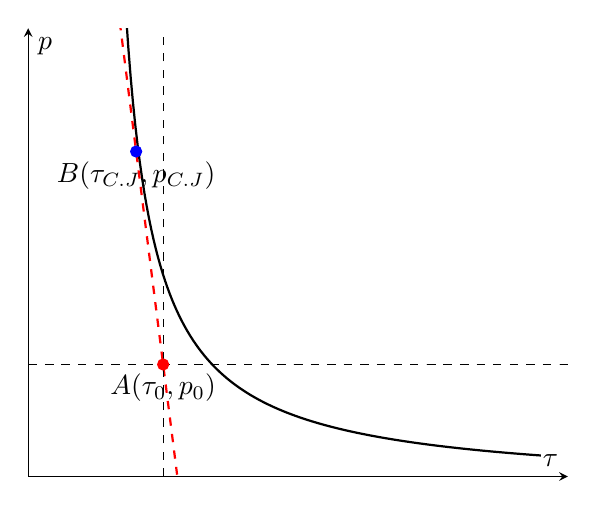
\begin{tikzpicture}
    \begin{axis}[
        domain=0.1:4,   % 设置 tau 的范围,略过 tau = 0.1667 的奇异点
        samples=200,     % 采样点数
        xlabel={$ \tau $},
        ylabel={$ p $},
        axis lines=middle,
        xmin=0, xmax=4,
        ymin=0, ymax=4,
        xtick=\empty,    % 去掉刻度标签
        ytick=\empty,    % 去掉刻度标签
        restrict y to domain=0:10,  % 限制 p 的范围
        no markers,      % 取消默认标记
        grid=none        % 不显示网格
    ]
    
    % 绘制 p = (10.3334 - 0.8164*tau) / (tau - 0.1667) 的曲线
    \addplot [
        domain=0.4:3.8,   % 从 tau = 0.2 开始,避开 tau = 0.1667 的奇异点
        thick,
        black
    ]
    {(1-0.1*x) / (x - 0.5)};
    \addplot [
      domain=0.4:1.2,   % 从 tau = 0.2 开始,避开 tau = 0.1667 的奇异点
      dashed,
      thick,
      red
  ]
  {-9.5*(x-1)+1};
  %   \addplot [
  %     domain=0.8:1.4,  
  %     thick,
  %     mark=square,
  %     mark repeat=40,  % 每隔一定距离放置一个标记
  %     mark size=1pt,  % 标记的大小
  %     only marks,      % 只画标记,不画连续的线
  %     black
  % ]
  % {(1-0.05*x) / (x - 0.25)};
    \addplot[
      domain=0.0:4,
      dashed
    ]
    {
      1.0
    };
    \addplot [
      dashed
  ] coordinates {(1.0, 0) (1.0, 4)};
    % 标记 tau_0 = 5, p_0 = 2 的点
    \addplot[
        only marks,
        mark=*,
        mark size=2pt,
        red
    ] coordinates {(1.0, 1.0)};
    \addplot[
      only marks,
      mark=*,
      mark size=2pt,
      blue
  ] coordinates {(0.8, 2.9)};
  \node at (axis cs:0.8,2.9) [anchor=north] {$B(\tau_{C.J}, p_{C.J})$};
    % 为点 (5, 2) 添加标签 tau_0, p_0
    \node at (axis cs:1.0,1.0) [anchor=north] {$A(\tau_0, p_0)$};
    \end{axis}
  \end{tikzpicture}
  \caption{The Crussard curve (black) and the Rayleigh line (red).}
  \label{fig:crussard}
\end{figure}



\begin{lemma}
  Along the Crussard curve, the detonation (resp. the deflagration) speed $|v_0|$ is local minimum (resp. maximum) for a C.J. detonation (resp. deflagration).
  Moreover, for a C.J. process, the speed $|v_1|$ of the burnt gas relative to the front is equal to the local sound speed, i.e.,
  \begin{equation}
    |v_1|=c_1 \text{ at C.J. points}.
  \end{equation}
\end{lemma}
The pressure of the C.J. point can be determined by the unburnt state and the heat of reaction $\Delta$. From \eqref{eq:M2}, we have
\begin{equation}
  \frac{p_1-p_0}{\tau_1-\tau_0} = -\rho_1^2v_1^2 = -\frac{\gamma p_1}{\tau_1}.
\end{equation}
We get the expression of $\tau_1$,
\begin{equation}
\tau_1 = \frac{\gamma \tau_0 p_1}{(1+\gamma)p_1-p_0}.
\end{equation}
Put this term into \eqref{eq:ideal_hugoniot}, we get
\begin{equation}
p_1^2 + 2ap_1 + b = 0,
\end{equation}
where, 
\[
a = -p_0 + \Delta (\gamma -1 ) \rho_0, \quad b = p_0^2 - 2\Delta \mu^2 \rho_0 p_0.
\]
Solve this quadratic equation, we get the pressure of the C.J. point,
\begin{equation}
  p_{CJ} = p_0 - (\gamma -1) \Delta \rho_0
  \left(1\pm \sqrt{1- \frac{2\gamma p_0}{(\gamma^2-1)\rho_0 \Delta}}\right).
\end{equation}
where, $+$ for the detonation branch and $-$ for the deflagration branch.
From $p_{CJ}$ expression, we get density of the C.J. point,
\begin{equation}
\rho_{CJ} = \frac{\rho_0\left(p_{CJ}(1+\gamma)-p_0 \right)}{\gamma p_{CJ}},
\end{equation}
and speed of the C.J. point,
\begin{equation}
 u_{CJ} = u_0 + (p_{CJ}-p_0)\sqrt{\frac{(1-\mu^2)\tau_0-2\mu^2 \Delta (p_0-p_{CJ})^{-1}}{\mu^2p_0+p_{CJ}}}.
\end{equation}

The more detailed analysis of the combustion wave can be found in \cite{tengRiemannProblemsReacting1982,godlewskiNumericalApproximationHyperbolic1996}.

\section{Wave Structure for the Reactive Riemann Problem}
The initial states for the reactive Riemann problem are denoted by $\boldsymbol{U}_L$ and $\boldsymbol{U}_R$, representing the left and right states, respectively. The variables in the regions between the waves are commonly referred to as the star states, while the two intermediate regions are called the star region in the literature. To maintain consistency with {\bf Sec.2}, we denote $\boldsymbol{U}_0$ and $\boldsymbol{U}_1$ as the states corresponding to the unburnt and burnt gases, respectively, in the frame of reference relative to the combustion front. Without loss of generality, we assume that the combustion front lies on the right of the contact discontinuity.

The wave structure for the reactive Riemann problem can be classified into the following four distinct cases, as illustrated in Figure \ref{fig:rp}:
\begin{enumerate}
  \item Strong Detonation.
  In the case of a strong detonation, the left wave is a genuinely non-linear wave, which may be either a shock or a rarefaction wave. We refer to this wave as the left genuinely non-linear (LGNL) wave. The middle wave is a contact discontinuity (CD), and the right wave is a strong detonation (SDT) wave.
  \[
  \boldsymbol{U}_L 
  \xrightarrow{\text{LGNL}}
  \boldsymbol{U}_L^*
  \xrightarrow{\text{CD}}
  \boldsymbol{U}_R^* (\boldsymbol{U}_1)
  \xrightarrow{\text{SDT}}
  \boldsymbol{U}_R (\boldsymbol{U}_0).
  \]

  \item CJ Detonation.
  In the case of a Chapman-Jouguet (CJ) detonation, the structure is similar to the strong detonation, but there is a composite wave between the middle and right states. This composite wave consists of a right rarefaction wave (RRW) followed by a CJ detonation (CJDT) wave.
  \[
    \boldsymbol{U}_L 
  \xrightarrow{\text{LGNL}}
  \boldsymbol{U}_L^*
  \xrightarrow{\text{CD}}
  \boldsymbol{U}_R^* (\boldsymbol{U}_1)
  \xrightarrow{\text{RRW}}
  \boldsymbol{U}_{CJ}
  \xrightarrow{\text{CJDT}}
  \boldsymbol{U}_R (\boldsymbol{U}_0).
  \]
  \item Weak Deflagration.
  In the case of a weak deflagration, the flow of gas relative to the combustion front is subsonic ahead of the front. As a result, the right genuinely non-linear (RGNL) wave appears on the right side of the deflagration wave.
  \[
    \boldsymbol{U}_L 
    \xrightarrow{\text{LGNL}}
    \boldsymbol{U}_L^*
    \xrightarrow{\text{CD}}
    \boldsymbol{U}_R^* (\boldsymbol{U}_1)
    \xrightarrow{\text{WDF}}
    \boldsymbol{U}_R^{**} (\boldsymbol{U}_0)
    \xrightarrow{\text{RGNL}}
    \boldsymbol{U}_R.
    \]
  \item CJ Deflagration.
  Similar to the CJ detonation, the CJ deflagration case also involves a composite wave between the middle and right states. This composite wave consists of a right rarefaction wave (RRW) followed by a CJ deflagration (CJDF) wave.
  \[
    \boldsymbol{U}_L 
    \xrightarrow{\text{LGNL}}
    \boldsymbol{U}_L^*
    \xrightarrow{\text{CD}}
    \boldsymbol{U}_R^* (\boldsymbol{U}_1)
    \xrightarrow{RR}
    \boldsymbol{U}_{CJ}
    \xrightarrow{\text{CJDF}}
    \boldsymbol{U}_R^{**} (\boldsymbol{U}_0)
    \xrightarrow{\text{RGNL}}
    \boldsymbol{U}_R.
    \]
\end{enumerate}
\begin{figure}[!htbp]
\centering
\subcaptionbox{Strong detonation}[0.45\textwidth]{
  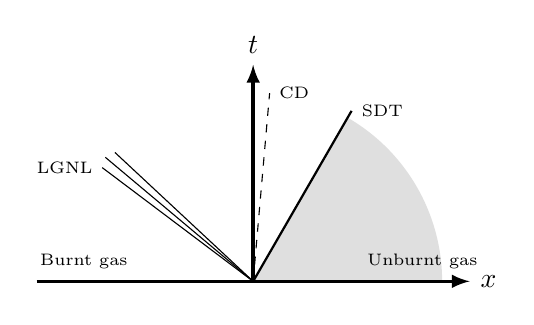
\begin{tikzpicture}[scale=.5]
    \tikzset{font={\fontsize{6pt}{10}\selectfont}}
    \fill [lightgray,opacity=.5] (0,0)--(4.8,0) arc(0:60:4.8);
    \draw[-latex,very thick](-5.5,0)--(5.5,0)
     node[right]{\normalsize $x$};
    \draw[-latex,very thick] (0,0)--(0,5.5)
  node[above] {\normalsize $t$};
    % \draw (2.7,0.3) node{$\bm U_r$};
    % \draw (-2.7,0.3) node{$\bm U_l$};
    % \draw (1.0,1.8) node{$\bm U_r^*$}; node[above]{\it $\bm{\mathcal W}_l$}
    % \draw (-1,1.5) node{$\bm U_l^*$}; node[above]{\it $\bm{\mathcal W}_r$}
    \draw [thick](0,0)--(60:5) node[right]{SDT};
    \draw (0,0)--(140:4.9);
    \draw (0,0)--(143:4.8) node[left]{LGNL};
    \draw (0,0)--(137:4.8);
    \draw[dashed] (0,0)--(85:4.8) node[right]{CD};
    \draw (4.3,0.5) node{Unburnt gas};
    \draw (-4.3,0.5) node{Burnt gas};
    \end{tikzpicture}
}
\hfil
\subcaptionbox{CJ detonation}[0.45\textwidth]{
  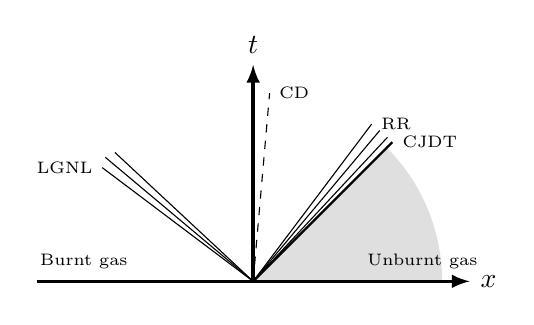
\begin{tikzpicture}[scale=.5]
    \tikzset{font={\fontsize{6pt}{10}\selectfont}}
    \fill [lightgray,opacity=.5] (0,0)--(4.8,0) arc(0:45:4.8);
    \draw[-latex,very thick](-5.5,0)--(5.5,0)
     node[right]{\normalsize $x$};
    \draw[-latex,very thick] (0,0)--(0,5.5)
  node[above] {\normalsize $t$};
    % \draw (2.7,0.3) node{$\bm U_r$};
    % \draw (-2.7,0.3) node{$\bm U_l$};
    % \draw (1.0,1.8) node{$\bm U_r^*$}; node[above]{\it $\bm{\mathcal W}_l$}
    % \draw (-1,1.5) node{$\bm U_l^*$}; node[above]{\it $\bm{\mathcal W}_r$}
    \draw [thick](0,0)--(45:5) node[right]{CJDT};
    \draw (0,0)--(47:5.0);
    \draw (0,0)--(50:5.0);
    \draw (0,0)--(53:5.0)node[right]{RR};
    \draw (0,0)--(140:4.9);
    \draw (0,0)--(143:4.8) node[left]{LGNL};
    \draw (0,0)--(137:4.8);
    \draw[dashed] (0,0)--(85:4.8) node[right]{CD};
    \draw (4.3,0.5) node{Unburnt gas};
    \draw (-4.3,0.5) node{Burnt gas};
    \end{tikzpicture}
}

\vspace{1em}

\subcaptionbox{Weak deflagration}[0.45\textwidth]{
  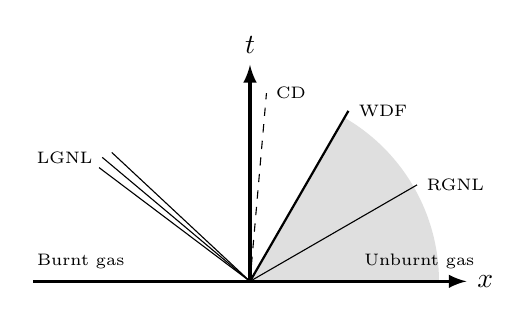
\begin{tikzpicture}[scale=.5]
  \tikzset{font={\fontsize{6pt}{10}\selectfont}}
  \fill [lightgray,opacity=.5] (0,0)--(4.8,0) arc(0:60:4.8);
  \draw[-latex,very thick](-5.5,0)--(5.5,0)
   node[right]{\normalsize $x$};
  \draw[-latex,very thick] (0,0)--(0,5.5)
node[above] {\normalsize $t$};
  % \draw (2.7,0.3) node{$\bm U_r$};
  % \draw (-2.7,0.3) node{$\bm U_l$};
  % \draw (1.0,1.8) node{$\bm U_r^*$}; node[above]{\it $\bm{\mathcal W}_l$}
  % \draw (-1,1.5) node{$\bm U_l^*$}; node[above]{\it $\bm{\mathcal W}_r$}
  \draw [thick](0,0)--(60:5) node[right]{WDF};
  \draw (0,0)--(30:4.9) node[right]{RGNL};
  \draw (0,0)--(140:4.9) node[left]{LGNL};
  \draw (0,0)--(143:4.8);
  \draw (0,0)--(137:4.8);
  \draw[dashed] (0,0)--(85:4.8) node[right]{CD};
  \draw (4.3,0.5) node{Unburnt gas};
  \draw (-4.3,0.5) node{Burnt gas};
  \end{tikzpicture}}
\hfil
\subcaptionbox{CJ deflagration}[0.45\textwidth]{
  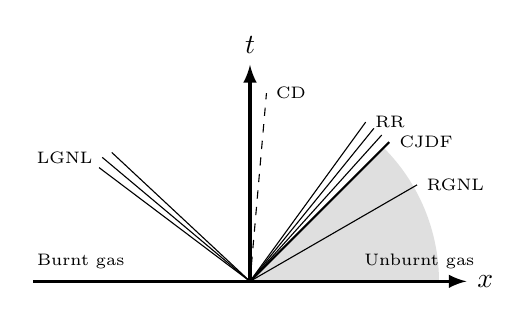
\begin{tikzpicture}[scale=.5]
   \tikzset{font={\fontsize{6pt}{10}\selectfont}}
    \fill [lightgray,opacity=.5] (0,0)--(4.8,0) arc(0:45:4.8);
    \draw[-latex,very thick](-5.5,0)--(5.5,0)
     node[right]{\normalsize $x$};
    \draw[-latex,very thick] (0,0)--(0,5.5)
  node[above] {\normalsize $t$};
    % \draw (2.7,0.3) node{$\bm U_r$};
    % \draw (-2.7,0.3) node{$\bm U_l$};
    % \draw (1.0,1.8) node{$\bm U_r^*$}; node[above]{\it $\bm{\mathcal W}_l$}
    % \draw (-1,1.5) node{$\bm U_l^*$}; node[above]{\it $\bm{\mathcal W}_r$}
    \draw [thick](0,0)--(45:5) node[right]{CJDF};
    \draw (0,0)--(30:4.9) node[right]{RGNL};
    \draw (0,0)--(48:5.0);
    \draw (0,0)--(51:5.0);
    \draw (0,0)--(54:5.0) node[right]{RR};
    \draw (0,0)--(140:4.9) node[left]{LGNL};
    \draw (0,0)--(143:4.8);
    \draw (0,0)--(137:4.8);
    \draw[dashed] (0,0)--(85:4.8) node[right]{CD};
    \draw (4.3,0.5) node{Unburnt gas};
    \draw (-4.3,0.5) node{Burnt gas};
    \end{tikzpicture}
}
  \caption{The Riemann problem for the reactive flow.
  LGNL: left non-linear wave; RGNL: right non-linear wave; CD: contact discontinuity; SDT: strong detonation; CJDT: CJ detonation; WDF: weak deflagration; CJDF: CJ deflagration; RR: right rarefaction wave.\label{fig:rp}}
\end{figure}


\section{Equations for Pressure and Velocity}

\section{Numerical Solution for Pressure}

\section{The Complete Solution}
\input{chapter/part3.tex}
\bibliographystyle{unsrt}
\bibliography{ReactiveFlow}

\end{document}
